%equations, bib. \\

This chapter provides the background theory for the project. First we give an overview of procedural generation and some of the different methods used in procedural generation. Then we give an overview of some basic music theory that is necessary to fully grasp the structure of the system. Then I will cover object oriented programming and then the concept of iterative development. Lastly I will cover the use of \ac{AI} in software development.

\section{Procedural generation}
\ac{PCG}, often reffered to as just \ac{PG}, is algorithmic generation of content. This content can take many forms including landscape, levels, textures or even 3D models. This leads to smaller file sizes since the program can generate the content using algorithms rather than having everything pre-made and saved. 

  This section will cover several methods of \ac{PG} and discuss similarities, differences and most importantly limitations of the methods. Additionally we will take a look at and what we are trying to achieve with the procedural generation in this project and propose a new method that will handle the problem of music generation in a new way. 

  \subsection{L-systems (Lindenmayer systems)}
  \textbf{\color{red}WIP section}\\
    Lindenmayer systems are a method of \ac{PG} based around the idea of creating rules for the generation which lead to self-similarity and fractal-like forms. This kind of \ac{PG} is often used in generating organic structures such as trees or other plant-like structures.

    If we observe Figure~\ref{fig:l_systems} we can see how two different L-systems can create both very rigid results in the form of the sierpinsky triangle and more organic structures like the fractal plant on the second line.

    \begin{figure}[h] % Sierpinksy and plant
      \begin{tabular}{ccc}

        
\includegraphics[width=0.3\textwidth]{figures/04theory/sierpinski1.png} &
        
\includegraphics[width=0.3\textwidth]{figures/04theory/sierpinski3.png} &
        
\includegraphics[width=0.3\textwidth]{figures/04theory/sierpinski5.png} \\
        & (a) sierpinksi triangle & \\
      
        
\includegraphics[width=0.3\textwidth]{figures/04theory/plant1.png} &
        
\includegraphics[width=0.3\textwidth]{figures/04theory/plant3.png} &
        
\includegraphics[width=0.3\textwidth]{figures/04theory/plant5.png} \\
        & (b) fractal plant & \\

        
\includegraphics[width=0.3\textwidth]{figures/04theory/bush1.png} &
        
\includegraphics[width=0.3\textwidth]{figures/04theory/bush3.png} &
        
\includegraphics[width=0.3\textwidth]{figures/04theory/bush5.png} \\
        & (c) fractal bush & \\

      \end{tabular}

      \caption{Demonstration of the sierpinski triangle, a fractal plant and bush after one, three and five iterations repsectively.}\label{fig:l_systems}
    \end{figure}

    \begin{figure}[h] % Arrowhead sierpinski
      \begin{tabular}{ccc}

        
\includegraphics[width=0.3\textwidth]{figures/04theory/arrowhead1.png} &
        
\includegraphics[width=0.3\textwidth]{figures/04theory/arrowhead2.png} &
        
\includegraphics[width=0.3\textwidth]{figures/04theory/arrowhead3.png} \\
        (a) first iteration & (b) second iteration & (c) third iteration \\
        
\includegraphics[width=0.3\textwidth]{figures/04theory/arrowhead4.png} &
        
\includegraphics[width=0.3\textwidth]{figures/04theory/arrowhead5.png} &
        
\includegraphics[width=0.3\textwidth]{figures/04theory/arrowhead6.png} \\
        (d) fourth iteration & (e) fifth iterations & (f) sixth iteration \\

      \end{tabular}
      \caption{Approximation of the sierpinski triangle using the sierpinski arrowhead curve.}\label{fig:arrowhead_sierpinski}
    \end{figure}

  \subsection{PG using constraint satisfaction}
  \textbf{\color{red}WIP section}\\
    Similar to \ac{WFC} we have \ac{PG} using constraint satisfaction. This method uses given constraints for influencing the generation. It usually works by randomly generating something in the given domain, then iterates over the generated data and enforces constraints in order to make it adhere to a model designed by the programmer or end user. After several iteration over the domain we end up with a domain where the constraints are satisfied for all the objects in the domain.


    In Figure~\ref{fig:cons_adjacent} you can see how the constraints are set up for this example, and Figure~\ref{fig:domain_prop} shows the initial domain with how many different states are left for each cell in the domain as well as the domain after AC-3 propagation. Finally Figure~\ref{fig:cs_solution} shows the final domain that satisfies both the local and the global constraints. 

    \begin{figure}[h] % Nodes
      \begin{center}
        
\includegraphics[width=0.95\textwidth]{figures/04theory/01_adjacency_constraints.pdf}
      \end{center}
      \caption{All different node types and how they are constrained. Each edge represents which note types can be adjacent in the domain.}\label{fig:cons_adjacent}
    \end{figure}

    \begin{figure}[h] % Initial domain and AC-3
      \begin{center}
        
\includegraphics[width=0.95\textwidth]{figures/04theory/02_domain_propagation.pdf}
      \end{center}
      \caption{Initial domain and domain after AC-3 propagation. The AC-3 algoriths reduces the search space by ensuring arc consistency.}\label{fig:domain_prop}
    \end{figure}

    \begin{figure}[h] % Final map
      \begin{center}
        
\includegraphics[width=0.6\textwidth]{figures/04theory/03_generated_solution.pdf}
      \end{center}
      \caption{Final generated map satisfying all constraints.}\label{fig:cs_solution}
    \end{figure}

  \subsection{Wave function collapse}
    \ac{WFC} is a method used to procedurally generate using either given constraints, or it can also use some input that it analyses and generates the constraints procedurally which are then used to generate something in the same style as the input. 

    It works by initializing the entire space in a superposition which means that the state is yet to be determined. We call this an \textit{unobserved} state, meaning we don't know what state it is in yet. These unobserved states are not complex numbers like they are in \ac{QM}, but the process is similar which is why it gets its name inspired by the field of \ac{QM}. Randomly assigning parts of the space we are able to collapse\footnote{collapsing a superposition means that we decide the actual state of the given position in the space} some of the \textit{wave function}\footnote{the wave function is simply the constraints what decide what the state of the object should be dependent on external factors}.
    
    The rules for how the tiling should propagate are derived from an example input. In Figure~\ref{fig:exemplar_and_rules} we see how from the simple input image the algorithm determines some local tiling rules for the different states and uses this as a basis for generating the new content. These generated rules are what make the output consistently similar and ensures we are outputting something that resembles the original input.

    \begin{figure}[h]
      \centering
        
\includegraphics[width=0.95\textwidth]{figures/04theory/01_exemplar_and_rules.pdf}
      \caption{Given the exemplar on the left the \ac{WFC} algorithm learns the local tile rules shown on the right.}\label{fig:exemplar_and_rules}
    \end{figure}

    In Figure~\ref{fig:observe_propagate_steps} we can see how the number of possible states reduces as soon as a state is collapsed. This propagets outward and the process of assigning states continues until the entire domain has collapsed.

    \begin{figure}[h]
      \centering
        \begin{tabular}{cc}
          
\includegraphics[width=0.4\textwidth]{figures/04theory/02_initial_wave.pdf} &
          
\includegraphics[width=0.4\textwidth]{figures/04theory/02_after_first_collapse.pdf} \\
          (a) initial wave & (b) after first collapse \\
          
\includegraphics[width=0.4\textwidth]{figures/04theory/02_after_propagation.pdf} &
          
\includegraphics[width=0.4\textwidth]{figures/04theory/02_complete_collapse.pdf} \\
          (c) after propagation & (d) compete collapse
        \end{tabular}
      \caption{Shows how collapsing/observing a state propagates. An observation reduces the local uncertainty.}\label{fig:observe_propagate_steps}
    \end{figure}

    
    When the rules for the tiling have been established we can use them to generate new examples, in Figure~\ref{fig:generated_wfc_map} we are able to generate a larger domain using the same rules we got from the example image.

    \begin{figure}[h]
      \begin{center}
        
\includegraphics[width=0.65\textwidth]{figures/04theory/03_generated_wfc_map.pdf}
      \end{center}
      \caption{An example output for a larger domain than the original exemplar. The consistent rules lead to consistently similar outputs.}\label{fig:generated_wfc_map}
    \end{figure}

    Finally we can see how the rules does not make it so that there is simply one output, we can change the seed for generation and end up with very different results, but all adhering to the initial rules derived from the exemplar in the very first step. 

    \begin{figure}[h]
      \begin{center}
        
\includegraphics[width=0.95\textwidth]{figures/04theory/04_seed_variations.pdf}
      \end{center}
      \caption{Illustration that the learned rules stay consistend while the seed changes the output.}\label{fig:wfc_seed_variations}
    \end{figure}
  
  \subsection{Binary space partitioning}
  \textbf{\color{red}WIP section}\\
    \ac{BSP} can be used to generate map layouts like indoor environments, in the following figures you can see an example of how we can divide the entire domain into sections and used that to generate rooms.
  
    \begin{figure}[h] % Initial partitioning
      \begin{center}
        
\includegraphics[width=0.5\textwidth]{figures/04theory/01_bsp_partitions.pdf}
      \end{center}
      \caption{Initial domain partitioning, made by recursively divinging the domain in two.}\label{fig:bsp_partitions}
    \end{figure}
    
    \begin{figure}[h] % Rooms and corridors
      \begin{center}
        
\includegraphics[width=0.5\textwidth]{figures/04theory/02_rooms_and_corridors.pdf}
      \end{center}
      \caption{Generated rooms inside the partitions and connected them with corridors between rooms.}\label{fig:rooms_and_corridors}
    \end{figure}

    \begin{figure}[h]
      \begin{center}
        
\includegraphics[width=0.5\textwidth]{figures/04theory/03_final_bsp_dungeon.pdf}
      \end{center}
      \caption{Rasterization of the generated dungeoun to show "final product".}\label{fig:final_bsp_dungeoun}
    \end{figure}

  \subsection{Random noise and seeds}
  \textbf{\color{red}WIP section}\\
    Perlin noise is a very common way to generate structures like worlds etc... It is very good at creating smooth transitions from one state to another, like height maps.
    This is demonstrated in the following figures below with some different techniques.
    
    \begin{figure}[h]
      \begin{center}
        
\includegraphics[width=0.95\textwidth]{figures/04theory/01_seed_variation.pdf}
      \end{center}
      \caption{}\label{fig:seed_variations}
    \end{figure}
    \begin{figure}[h]
      \begin{center}
        
\includegraphics[width=0.95\textwidth]{figures/04theory/02_noise_octaves.pdf}
      \end{center}
      \caption{}\label{fig:noise_octaves}
    \end{figure}
    \begin{figure}[h]
      \begin{center}
        
\includegraphics[width=0.95\textwidth]{figures/04theory/03_noise_to_terrain.pdf}
      \end{center}
      \caption{}\label{fig:noise_to_terrain}
    \end{figure}
    \begin{figure}[h]
      \begin{center}
        
\includegraphics[width=0.95\textwidth]{figures/04theory/04_parameter_control.pdf}
      \end{center}
      \caption{}\label{fig:parameter_control}
    \end{figure}

  \subsection{Random walks}
    Random walk procedural generation method that can be used to organic looking structures like maps and textures. It can also be used to describe natural phenomena like bacterial movement. It has been applied in financial economics and computer science

    The random walk works by having an entity walk around randomly. In some cases the random walk is also called the \textit{drunkard's walk}. Then the path is traced, either to create a circumference of an area or the traversed spaces become the area itself. Oftentimes the drunk walker has a set amount of time or steps it can walk before it is terminated, then a new walker is placed at a random location, this helps to smooth out the generated area.

    The same technique can be used to create textures as well, in Figure~\ref{fig:random_walks} we can see how changing the colours and directional bias we can generate textures that imitate real life. In the tree and sand example the directional bias is vertical for the tree texture and diagonal for the sand texture. For the map texture it is uniform directional bias, but colouring to indicate water, land and mountains. The least traveled to square get more blue, and the more frequent it goes to green and brown/white to indicate mountains.

    \begin{figure}[h]
      \centering
        
\includegraphics[width=0.32\textwidth]{figures/04theory/ex_wood.png}
        
\includegraphics[width=0.32\textwidth]{figures/04theory/ex_sand.png}
        
\includegraphics[width=0.32\textwidth]{figures/04theory/ex_map.png}
      \caption{Three different textures generated using random walks.}\label{fig:random_walks}
    \end{figure}

  \subsection{Discussion}
  \textbf{\color{red}WIP section}\\
    Now that we have taken a look into a few methods of \ac{PG} we observe that there are many similarities between the methods. Common for all forms of \ac{PG} is that they utilize some form of randomness. The randomness in a core part of procedural generation, if there was no randomness we would generate the same output every time and that would be the same as just creating the content yourself.


\clearpage{}
\section{Music theory}
  This section contains some basic music theory relevant for understanding how music is constructed. It is not necessary to understand everything in depth, but familiarity with these concepts will be of great help when reading the musical parts of the thesis. Throughout the thesis there are several examples and figures using musical notation, so a basic understanding of how to read them is beneficial.

  \subsection{Notes}
    The very core of music is sound. Sounds are vibrations in air which we interpret as pitches if the oscillation is somewhat stable. In the western system the standard reference pitch is \musPitch{A}{4}, which is $440$ Hz. The subscript four indicates the fourth octave. All other pitches are tuned in relation to this reference.

    The musical note is represented on the staff by a circular symbol called the note-head. The vertical placement of the note-head on the staff determines which pitch it represents. This is illustrated in Figure~\ref{fig:piano-notes}, where we can see the placement of the notes from \musPitch{C}{2} up to \musPitch{C}{5}. Notice how only the white keys from the piano are notated directly. The black keys are notated with the \musSharp- and \musFlat-symbols. The \musSharp-symbol is pronounced "sharp" and raises the note by a semitone, and the \musFlat-symbol is pronounced "flat" and lowers the note by a semitone\footnote{a semitone is the smallest musical interval and it is the distance between two adjacent notes}. The horizontal placement is not directly an indication of time or duration; the temporal aspect is instead defined symbolically. The note can also have a stem, which is a vertical line attached to the note-head. The direction of the stem (up or down) does not change the pitch, but it can affect the visual layout of the music.

    \begin{figure}[h]
      \begin{center}
        
\includegraphics[trim={0.8cm 8cm 1.1cm 3.1cm}, clip, width=1\textwidth]{figures/04theory/Piano-notes.pdf}
      \end{center}
      \caption{Overview of note placement on the staff and piano.}\label{fig:piano-notes}
    \end{figure}

    The same musical pitch can be written in several different ways in order to indicate the duration of the note. This is done by using variations of the stem and notehead. In Figure~\ref{fig:note-value} the different parts of the note are highlighted with colour. The note-head is black, and its placement decides which musical pitch is represented. The stem can go either up or down; this does not change the meaning, it only makes the notation more compact when the note is placed high or low on the staff. The direction of the stem can also carry meaning if two notes occur simultaneously on one staff, since it usually indicates two different voices.
    Next we have the beams and the flags coloured in purple and blue respectively. These two carry the same meaning: one flag is equivalent to one beam, meaning they represent the same duration. The beam simply makes the notation less visually crowded when reading.
    The duration symbolized by the flag and beam can be seen in Table~\ref{tab:note-values} and Figure~\ref{fig:notevalues}. These are not exhaustive, since we can alter these durations in several ways, but they are sufficient for the scope of this thesis.

    \begin{figure}[h] % Note values
      \begin{center}
        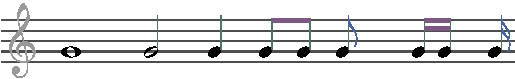
\includegraphics[trim={1cm 0cm 0cm 0cm}, clip, width=0.95\textwidth]{examples/04theory/09-value.cropped.pdf}
      \end{center}
      \caption{The figure shows the parts of the musical note. The note-head in black, stem in green, beam in purple and flag in blue.}\label{fig:note-value}
    \end{figure}

    \begin{table}[h] % Table note values
      \NewDocumentCommand{\musWholeRest} {}{\musFont{\symbol{11}}}
      \NewDocumentCommand{\musHalfRest} {}{\musFont{\symbol{10}}}
      \NewDocumentCommand{\musQuarterRest} {}{\musFont{\symbol{62}}}
      \NewDocumentCommand{\musEightRest} {}{\musFont{\symbol{63}}}
      \NewDocumentCommand{\musSixteenthRest} {}{\musFont{\symbol{64}}}
      \NewDocumentCommand{\musThirtySecondRest} {}{\musFont{\symbol{65}}}
      \caption{Table with common note values, their names and their corresponding duration.}\label{tab:note-values}
      \begin{center}
        \begin{tabular}[c]{|c|l|c|l|}
          \hline
          \multicolumn{1}{|c|}{\textbf{Symbol}} & 
          \multicolumn{1}{c|}{\textbf{Name}} & 
          \multicolumn{1}{c|}{\textbf{Rest symbol}} & 
          \multicolumn{1}{c|}{\textbf{Duration}} \\
          \hline
          \musWhole & Whole note & \musWholeRest & 4 beats \\
          \musHalf & Half note & \musHalfRest & 2 beats \\
          \musQuarter & Quarter note & \musQuarterRest & 1 beat\\
          \musEighth & Eighth note & \musEightRest & $\sfrac{1}{2}$ beat\\
          \musSixteenth & Sixteenth note & \musSixteenthRest & $\sfrac{1}{4}$ beat\\
          \musThirtySecond & Thirty-second note & \musThirtySecondRest & $\sfrac{1}{8}$ beat\\
          \hline
        \end{tabular}
      \end{center}
    \end{table}

    \begin{figure}[h] % Note values tree
      \begin{center}
      \begin{tikzpicture}[
        every node/.style={inner sep=2pt, scale=2},
        level1/.style={yshift=-2cm},
        level2/.style={yshift=-4cm},
        level3/.style={yshift=-6cm},
        every path/.style={->, shorten >=5pt, shorten <=5pt}]

        % --- Top ---
        \node (top) at (0,0) {\musWhole};

        % --- Level 2 ---
        \node (l2a) at (-2,-1) {\musHalf};
        \node (l2b) at ( 2,-1) {\musHalf};

        % --- Level 3 (spread evenly!) ---
        \node (l3a) at (-3,-3) {\musQuarter};
        \node (l3b) at (-1,-3) {\musQuarter};
        \node (l3c) at ( 1,-3) {\musQuarter};
        \node (l3d) at ( 3,-3) {\musQuarter};

        % --- Level 4 (8 notes, evenly spaced) ---
        \node (l4a) at (-3.5,-5) {\musEighth};
        \node (l4b) at (-2.5,-5) {\musEighth};
        \node (l4c) at (-1.5,-5) {\musEighth};
        \node (l4d) at (-0.5,-5) {\musEighth};
        \node (l4e) at ( 0.5,-5) {\musEighth};
        \node (l4f) at ( 1.5,-5) {\musEighth};
        \node (l4g) at ( 2.5,-5) {\musEighth};
        \node (l4h) at ( 3.5,-5) {\musEighth};

        % --- Arrows ---
        \draw[->] (top) -- (l2a);
        \draw[->] (top) -- (l2b);

        \draw[->] (l2a) -- (l3a);
        \draw[->] (l2a) -- (l3b);
        \draw[->] (l2b) -- (l3c);
        \draw[->] (l2b) -- (l3d);

        \draw[->] (l3a) -- (l4a);
        \draw[->] (l3a) -- (l4b);

        \draw[->] (l3b) -- (l4c);
        \draw[->] (l3b) -- (l4d);

        \draw[->] (l3c) -- (l4e);
        \draw[->] (l3c) -- (l4f);

        \draw[->] (l3d) -- (l4g);
        \draw[->] (l3d) -- (l4h);

      \end{tikzpicture}
      \end{center}
      \caption{Tree structure showing how the whole note can be divided into smaller note values. Each level in the tree takes the same amount of time, meaning the whole note at the top lasts as long as the eight eighth notes at the bottom.}
      \label{fig:notevalues}
    \end{figure}

  \subsection{Scales and Keys}\label{sec:keys}
    The musical scale is a building block for creating not only melodies but also harmony, which we will cover a bit later.
    Firstly, a musical scale is an ordered set of musical notes. In the western canon this is usually seven notes. You can see the basic C-major scale in Figure~\ref{fig:c-major-scale}; it is comprised of the notes \musPitch{C}{} \musPitch{D}{} \musPitch{E}{} \musPitch{F}{} \musPitch{G}{} \musPitch{A}{} \musPitch{B}{}. The tones of the scale can be named according to their function within the scale. We often label the notes \musDegree{1}, \musDegree{2}, \musDegree{3}, \musDegree{4}, \musDegree{5}, \musDegree{6}, \musDegree{7}, and then return to \musDegree{1}. Here the carets are used to distinguish scale degrees from the chord symbols that will be discussed in Section~\ref{sec:harmony}.
    We can also alter these degree numbers using the \musFlat- and \musSharp-symbols for instance the minor scale would be notated \musDegree{1}, \musDegree{2}, \musFlat\musDegree{3}, \musDegree{4}, \musDegree{5}, \musFlat\musDegree{6}, \musFlat\musDegree{7}. And the notes in the \musPitch{C}{}-minor scale would be \musPitch{C}{} \musPitch{D}{} \musPitch{E\fl}{} \musPitch{F}{} \musPitch{G}{} \musPitch{A\fl}{} \musPitch{B\fl}{}. The placement of the sharp- and flat-symbols before or after comes from the pronunciation of the notes, we say "flat three" and "sharp four", but we say "E flat" and "F sharp". 
    When we consider chord structures we use the numbers but usually count above from 8 to signify harmonic functions, but when considering only scales and melodies we usually only use 1 through 7.
    \newline

    The different notes in the scale have different functional names, and these names are not tied to the absolute pitch. Whether the note is \musPitch{C}{} or \musPitch{E\fl}{}, the functional name is the same as long as it is the same scale degree.
    \noindent The most important function is that of scale degree \musDegree{1}. This is the \textit{tonic}, which is the 'home' of the key. It is the most stable function and feels resolved, without any strong tension urging it to move elsewhere.
    In Table~\ref{tab:scale-degrees} you can see the common names for the scale degrees. These fancy names simply give some context to what functions the notes usually play in a melody. The leading tone has a lot of tension and wants to resolve to the tonic above.


    \begin{table}[h]
      \caption{Scale degrees and their functional names.}\label{tab:scale-degrees}
      \begin{center}
        \begin{tabular}[c]{|c|c|}
          \hline
          \textbf{Scale-Degree Number} & \textbf{Scale-Degree Name} \\
          \hline
           1 & Tonic \\
           2 & Supertonic \\
           3 & Mediant \\
           4 & Subdominant \\
           5 & Dominant \\
           6 & Submediant \\
           7 & Leading tone \\
          \hline
        \end{tabular}
      \end{center}
    \end{table}

    % C major scale
    \begin{example}[H]
      \begin{center}
        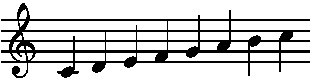
\includegraphics[width=0.8\textwidth]{examples/04theory/01-scale.cropped.pdf}
      \end{center}
      \caption[The \musPitch{C}{}-major scale written in the treble clef.]{The \musPitch{C}{}-major scale written in the treble clef. \examplelink.}
      \label{fig:c-major-scale}
    \end{example}

    % Eb major scale
    \begin{example}[H]
      \begin{center}
        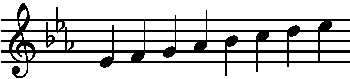
\includegraphics[width=0.8\textwidth]{examples/04theory/02-scale_eb.cropped.pdf}
      \end{center}
      \caption[The \musPitch{E\fl}{}-major scale written in the treble clef.]{The \musPitch{E\fl}{}-major scale written in the treble clef. \examplelink.}
      \label{fig:eb-major-scale}
    \end{example}

    The concept of a musical key is simply shifting where the tonic note is placed. For instance, in Example~\ref{fig:c-major-scale} you can see the major scale in \musPitch{C}{}, and Example~\ref{fig:eb-major-scale} shows the major scale in \musPitch{E\musFlat}{}. These two scales preserve the same intervallic relationships even though the actual pitches are different. The key is simply named after the tonic note, so the first example is in the key of \musPitch{C}{} major and the second example is in the key of \musPitch{E\fl}{} major. The concept of a key is important because it gives us a reference point for understanding the function of notes and chords within a piece of music. It also helps us understand how melodies and harmonies are constructed and how they relate to each other.

  % \subsection{Melodies}
  %   Melodies is the horizontal component of music, meaning we look at it as a time-series. We have a given note at a given length followed by another note or rest of a given length etc... This means that you can look at a melody as a series of intervals as well. If we do this on known melodies we will observe that they are mainly composed of steps and skips. This means that the distance between one note and the next is one or two tones. Large leaps are usually leaping to important tones like the tonic or the root of the current chord. 

  \subsection{Intervals}
    Before discussing harmony we need to consider the different types of distances between notes. The musical distance between two notes is called an \textit{interval}. Intervals can be identified by the number of semitones between the notes. All intervals have special names, and some distances can have different names depending on how they are spelled\footnote{the same pitch can be "spelled" in different ways, for instance \musPitch{A\fl}{} and \musPitch{G\musSharp}{} are written differently, but sound the same since they are the same pitch}. These names can be seen in Table~\ref{tab:intervals}, which also provides the number of semitones between the notes.

    In Figure~\ref{fig:normal_intervals} we can see how all the normal intervals look on a stave. Naming the interval starts by finding the general distance, meaning we first look at the note names. If we consider the interval between \musPitch{C}{} and \musPitch{E\fl}{}, we first observe that from \musPitch{C}{} to \musPitch{E}{} we count three letter names: \musPitch{C}{}, \musPitch{D}{}, and \musPitch{E}{}. This means we have some kind of third. We then look at the quality of that third. Since the \musPitch{E}{} is flattened to \musPitch{E\fl}{}, we have a minor third because the distance is 3 semitones instead of 4. You can see this in Example~\ref{fig:all_intervals}. There we observe that the distance between the notes in a minor third and a major third is the same in terms of letter names; the only difference is that the minor third is one semitone smaller, and that is shown by the \musFlat{}-symbol. Consequently, for the tritone we see that there are two ways to spell the same sounding interval: one is a fourth that has been raised and the other is a fifth that has been lowered. These two are \textit{enharmonically equivalent}, which means that they sound the same even though they are spelled differently. For the augmented fourth, which is the first spelling of the tritone shown here, we see the \musSharp{}-symbol used to indicate that the note has been raised by a semitone.


    \begin{table}
      \caption{Table containing all musical intervals up to an octave, the number of semitones and their abbreviated form.}\label{tab:intervals}
      \begin{center}
        \begin{tabular}[c]{|l|l|l|}
          \hline
          \multicolumn{1}{|c|}{\textbf{Interval name}} & 
          \multicolumn{1}{c|}{\textbf{Semitones}} &
          \multicolumn{1}{c|}{\textbf{Abbreviation}} \\
          \hline
          Unison & 0 & P1\\
          Minor second & 1 & m2 \\
          Major second & 2 & M2 \\
          Minor third & 3 & m3 \\
          Major third & 4 & M3 \\
          Perfect fourth & 5 & P4 \\
          Tritone\tablefootnote{can also be called diminished fifth or augmented fourth, where diminished simply means lowered by semitone and augmented means raised by one semitone} & 6 & TT or aug4/dim5\\
          Perfect fifth & 7 & P5 \\
          Minor sixth & 8 & m6 \\
          Major sixth & 9 & M6 \\
          Minor seventh & 10 & m7 \\
          Major seventh & 11 & M7 \\
          Octave & 12 & P8 \\
          
          \hline
        \end{tabular}
      \end{center}
    \end{table}

    \begin{figure}[H]
      \begin{center}
        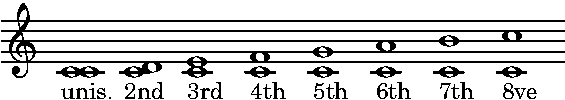
\includegraphics[width=0.95\textwidth]{examples/04theory/03-normal_intervals.cropped.pdf}
      \end{center}
      \caption{All normal intervals from the note \musPitch{C}{4} devoid their variants in quality.}\label{fig:normal_intervals}
    \end{figure}

    \begin{example}[H]
      \begin{center}
        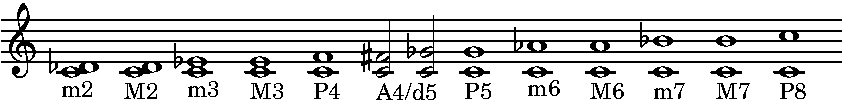
\includegraphics[width=0.95\textwidth]{examples/04theory/04-all_intervals.cropped.pdf}
      \end{center}
      \caption[All musical intervals from the unison to the octave, including their variants.]{All the musical intervals from the unison to the octave including their variants. \examplelink.}\label{fig:all_intervals}
    \end{example}
    
  \subsection{Harmony}\label{sec:harmony}
    Harmony is the vertical component of the music, meaning the notes that happen at the same time. When more than one note is played at the same time we call them chords.
    When considering harmonic progression in tonal music we can consider all the standard chords in the major key. They are labelled by Roman numerals. Upper case means the chord is major and lower case means it is minor. You can see the difference between major and minor chords in Example~\ref{fig:four_chords}, and hear the difference through the link provided in the caption. \\

    Example~\ref{fig:diatonic_chords_d_major} shows the full set of diatonic triads in D major\footnote{the $vii\deg$ means that it is a diminished chord, explanation can be seen in Figure~\ref{fig:four_chords}}. The Roman numerals make the chord quality clear, and the functional labels connect each triad to its role in the key. This is the harmonic material that forms the basis for the progression patterns discussed below.

    \begin{example}[h]
      \begin{center}
        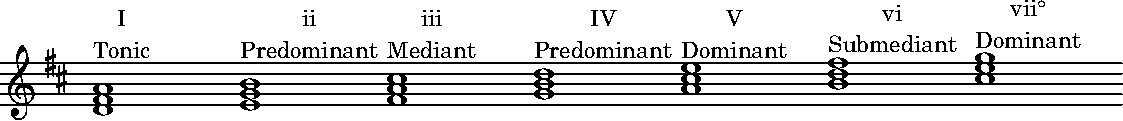
\includegraphics[width=0.98\textwidth]{examples/04theory/11-diatonic_chords.cropped.pdf}
      \end{center}
      \caption[The diatonic triads in D major with Roman numerals and functional names.]{The diatonic triads in D major with Roman numerals and functional names. \examplelink.}\label{fig:diatonic_chords_d_major}
    \end{example}

    Looking at Figure~\ref{fig:harmonic_progression} we can see the typical flow of harmonic functions in tonal music. Tonic means the home, the most stable function. Dominant is the function with the most tension. Pre-dominant usually leads into the dominant or sets the expectation for the dominant. The mediant and submediant are usually not considered part of the main harmonic progression, but they can be used to create interesting harmonic progressions and add some colour to the music. The arrows indicate the typical flow of harmonic functions, however this is not a strict rule. \\

    In harmonic context we often talk about cadences. Cadences classify how one harmony moves into another. The most common cadence is the \ac{PAC}, where we move from the dominant function to the tonic function, for instance from V to I. This is the most stable and resolved cadence, and it is the musical equivalent of a full stop in language. A closely related cadence is the \ac{IAC}, which also moves from dominant to tonic, but lacks some part of the full closure of a \ac{PAC}, for instance because the soprano does not end on the tonic or because one of the chords is inverted. Another common cadence is the \ac{HC}, where the phrase ends on the dominant, for instance by moving from IV to V. This creates tension and leaves us hanging on the dominant function, which usually leads back to the tonic. There are many other types of cadences, but these are among the most common ones. \cite{benCadencesMusicTheory2013} \\

    When writing music with harmonization we often restrict the individual melodies to certain ranges. This ensures that if the music is to be sung or played, the performer must be able to reach all the notes in the line. In traditional four-part harmony, the human voice is often used as the reference instrument, and the different vocal ranges have different names. From the highest voice to the lowest we have the \textit{soprano}, \textit{alto}, \textit{tenor}, and \textit{bass}. The soprano and alto voices are usually female voices, while the tenor and bass voices are usually male voices.
    When writing a harmonization we specify which voices are present. For instance, we can have an SATB harmonization, meaning all four standard voice types are present. We can also have TTBB, which means we have two tenor voices and two bass voices. This concept will be used when the generated melodies are harmonized later in the thesis.

    \begin{figure}[h]
      \centering
      \begin{tikzpicture}[
        node distance=1.8cm,
        every node/.style={font=\large},
        arrow/.style={-Latex, thick},
        box/.style={draw, thick, inner sep=6pt}
        ]

        % Main nodes
        \node (iii) {iii};
        \node[right=of iii] (vi) {vi};

        \node[right=of vi] (pre) {
            \begin{tabular}{c}
              ii\\
              IV
            \end{tabular}
          };

        \node[right=of pre] (dom) {
            \begin{tabular}{c}
              V\\
              vii$^\circ$
            \end{tabular}
          };

        \node[right=of dom] (I) {I};
        \node[right=0.8cm of I] (any) {ANY};
        
        \node[above=24pt of I] {\small Tonic};
        \node[above=24pt of iii] {\small Mediant};
        \node[above=24pt of vi] {\small Submediant};

        % Boxes around functional groups
        \node[box, fit=(pre)] (prebox) {};
        \node[above=4pt of prebox] {\small Pre-dominant};

        \node[box, fit=(dom)] (dombox) {};
        \node[above=4pt of dombox] {\small Dominant};

        % Arrows (horizontal)
        \draw[arrow] (iii) -- (vi);
        \draw[arrow] (vi) -- (prebox);
        \draw[arrow] (prebox) -- (dombox);
        \draw[arrow] (dombox) -- (I);
        \draw[arrow] (I) -- (any);

        % Curved return arrow
        \draw[arrow] 
          (dombox.south) 
          .. controls +(0,-1.5) and +(0,-1.5) .. 
          (iii.south);

      \end{tikzpicture}
      \caption{Harmonic progression in tonal music. The arrows indicate the typical flow of harmonic functions.}\label{fig:harmonic_progression}
    \end{figure}

    \begin{example}[h]
      \begin{center}
        
\includegraphics[width=0.95\textwidth]{examples/04theory/10-majmin.cropped.pdf}
      \end{center}
      \caption[The four main triads: major, minor, diminished, and augmented.]{The four main triads (chords with three notes): major, minor, diminished, and augmented. These are the most basic chord qualities, but major and minor are the most common ones. \examplelink.}\label{fig:four_chords}
    \end{example}
    
  \pagebreak{}
  \subsection{Time signatures}
    The time signature in a piece of music explains the temporal aspect, meaning it dictates how many of which duration fits into a single bar of music. A bar is the space between the vertical lines on the staff.
    A $4/4$ time signature, sometimes written as \meterC, means that there are four quarter notes per bar, and consequently $3/4$ time means that there are three quarter notes per bar. For this thesis I will only employ the standard $4/4$ time signature; it is the most common and straightforward time signature. Figure~\ref{fig:timesignatures} shows a few common time signatures. Notice how $4/4$ and $2/2$ contain the same total amount of time per bar, but the note values are grouped differently. This distinction affects how the music is subdivided and consequently how the rhythm is perceived and felt.

    \begin{figure}[H]
      \begin{center}
        
\includegraphics[width=0.95\textwidth]{examples/04theory/07-timesigs.cropped.pdf}
      \end{center}
      \caption{Demonstration of a few common time signatures and how the type of note is the lower number and the amount is the higher. For instance, $\frac{3}{4}$ has \textit{three} instances of the \textit{quarter} note. }\label{fig:timesignatures}
    \end{figure}

  \subsection{Musical form}
    Now that we have an idea of the musical structures on the melodic and harmonic layer we will take a look at musical forms. This is a very important idea when it comes to constructing melodies. A melody is not an infinitely wandering idea of music. A good melody follows a form. Often this can be viewed as repetitions and variations of a given musical idea. Two very common forms of musical form are the \textit{sentence form} and the \textit{period form}. \cite[pp.20-24]{shoenbergComposition}

    In Example~\ref{fig:sentence} we can see an example of the musical sentence. It starts with a 2-bar opening phrase labelled as the \textit{basic idea}, then we have a repetition of the same idea adapted to a new chord. The following 2 bars are a fragmentation of the idea. The last two bars form a conclusion, which ties the idea together. The cadence at the end can be considered the end of the sentence before the music moves on to something else.

    \begin{example}[H]
      \begin{center}
        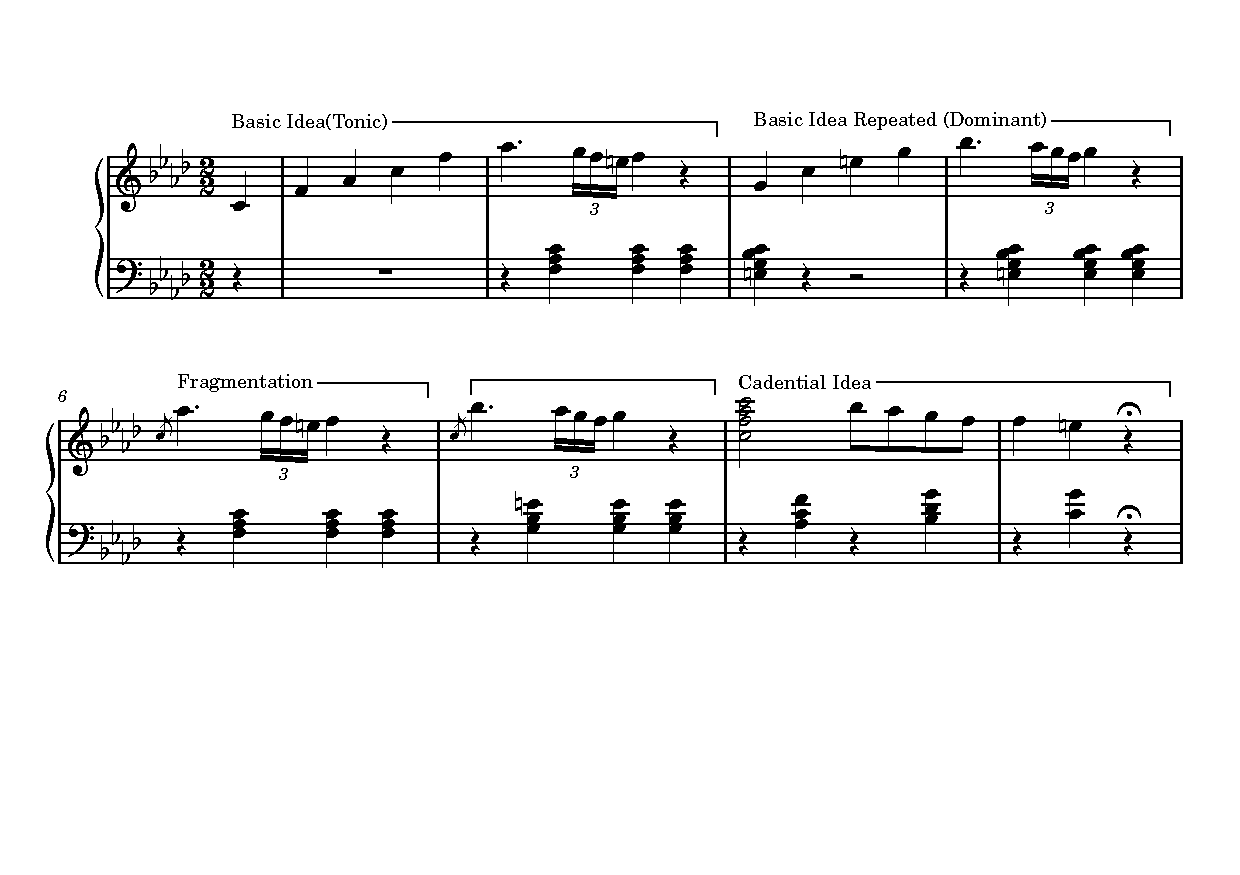
\includegraphics[width=1\textwidth]{examples/04theory/musical_sentence.cropped.pdf}
      \end{center}
      \caption[A classical example of the musical sentence form from the opening bars of Beethoven's piano sonata in F minor.]{A classical example of the musical sentence form. These are the opening bars of Beethoven's piano sonata in F minor \cite{SentenceMusic2023}. \examplelink}\label{fig:sentence}
    \end{example}

    In Example~\ref{fig:period} we see an example of the musical period. This example is from the British folk song \textit{Greensleeves}. The period is a form that is very similar to the sentence, but it has a more balanced structure. It consists of two phrases: the first one is called the \textit{antecedent} and the second one the \textit{consequent}. The antecedent phrase ends with a half cadence, which creates tension and leads us to the consequent phrase, which ends with a perfect authentic cadence and gives us a sense of closure\footnote{see Section~\ref{sec:harmony} for recap of cadences}.

    \begin{example}[H]
      \begin{center}
        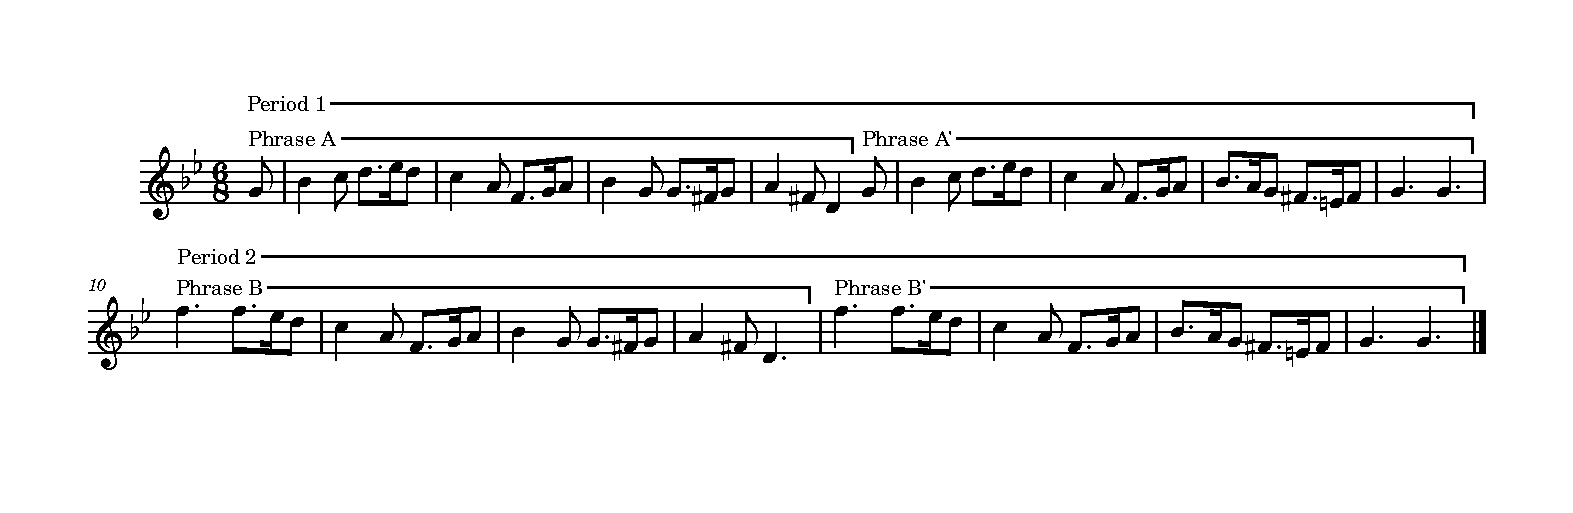
\includegraphics[width=1\textwidth]{examples/04theory/musical_period.cropped.pdf}
      \end{center}
      \caption[A classical example of the musical period form from the melody of the British folk song \textit{Greensleeves}.]{A classical example of the musical period form. This is the melody of the British folk song \textit{Greensleeves} \cite{PeriodMusic2025}. \examplelink}\label{fig:period}
    \end{example}


\clearpage{}
\section{Object oriented programming}

  \ac{OOP} is a way of structuring software around \textit{objects}. An object combines data and behaviour, meaning that it stores information and also provides operations that can act on that information. Instead of treating a program as one long sequence of instructions, the program is divided into units that represent meaningful concepts in the problem domain \cite{ObjectorientedProgramming2026,JacobsonOOSE}.

  In practical terms this usually means that the programmer defines a \textit{class}, which acts as a template, and then creates \textit{objects} from that class. Figure~\ref{fig:oop_class_object} illustrates this idea using a simple melody example. The class describes what information a melody should contain and what operations are available, while the object is one concrete melody with specific values.

  \begin{figure}[htbp]
  \centering
  \resizebox{0.92\textwidth}{!}{%
  \begin{tikzpicture}[
    >=Latex,
    font=\small,
    node distance=12mm and 14mm,
    classbox/.style={
      draw,
      rounded corners=3pt,
      minimum width=58mm,
      align=left,
      fill=blue!6
    },
    objectbox/.style={
      draw,
      rounded corners=3pt,
      minimum width=58mm,
      align=left,
      fill=green!7
    },
    arrow/.style={-{Latex[length=2.3mm]}, thick}
  ]
    \node[classbox] (class) {
      \textbf{Class: Melody}\\[1mm]
      Attributes:\\
      \quad title\\
      \quad events\\
      \quad key\\[1mm]
      Methods:\\
      \quad add\_event()\\
      \quad get\_length()
    };

    \node[objectbox, right=28mm of class] (object) {
      \textbf{Object: melody\_a}\\[1mm]
      title = ``Example theme''\\
      events = (c4, d4, e4, g4, \ldots)\\
      key = C major
    };

    \draw[arrow] (class) -- node[above, align=center] {instantiated as\\a concrete melody} (object);
  \end{tikzpicture}%
  }
  \caption{A simple illustration of the difference between a class and an object. A class describes what kind of data and behaviour an object has, while an object stores one concrete instance.}
  \label{fig:oop_class_object}
\end{figure}


\subsection{Encapsulation and abstraction}

  Two central ideas in \ac{OOP} are encapsulation and abstraction. Encapsulation means that related data and behaviour are grouped together. For example, instead of storing note events in one place and melody-related operations in another, they can be kept together in a single object. This makes the program easier to reason about because the responsibilities of each object become clearer.

  Encapsulation also makes it easier for an object to preserve its own consistency. If a melody should only be changed through well-defined operations such as adding an event, transposing the line, or exporting it, then the class can ensure that the internal data remains valid. Outside code does not need to know exactly how the events are stored in order to use the melody object safely.

  Abstraction means that a class can expose the parts of the system that are important for the user of the class, while hiding unnecessary implementation details. In a well-structured program this reduces complexity, because a developer can interact with a class through a small set of meaningful operations instead of having to understand every internal detail. In a music-related program this is especially useful because it allows the code to work with concepts such as melodies, motifs, and phrases directly instead of only with low-level pitch and duration lists. Figure~\ref{fig:oop_encapsulation_abstraction} illustrates this by separating a small public interface from the internal details stored inside the object.

  \begin{figure}[htbp]
  \centering
  \resizebox{0.95\textwidth}{!}{%
  \begin{tikzpicture}[
    >=Latex,
    font=\small,
    node distance=20mm and 14mm,
    outerbox/.style={
      draw,
      rounded corners=3pt,
      minimum width=78mm,
      minimum height=50mm,
      fill=gray!6
    },
    innerbox/.style={
      draw,
      rounded corners=3pt,
      minimum width=60mm,
      align=left
    },
    caller/.style={
      draw,
      rounded corners=3pt,
      minimum width=30mm,
      align=center,
      fill=blue!6
    },
    arrow/.style={-{Latex[length=2.3mm]}, thick}
  ]
    \node[caller] (user) {Other code};

    \node[outerbox, right=24mm of user] (melody) {};
    \node[anchor=north] at (melody.north) {\textbf{Melody object}};

    \node[innerbox, fill=green!8, anchor=north] (public) at ([yshift=-6mm]melody.north) {
      \textbf{Public operations}\\
      \quad add\_event()\\
      \quad transpose()\\
      \quad to\_lilypond()
    };

    \node[innerbox, fill=yellow!10, anchor=south] (internal) at ([yshift=2mm]melody.south) {
      \textbf{Internal details}\\
      \quad events\\
      \quad cached length\\
      \quad harmony references
    };

    \draw[arrow] (user) -- node[above] {uses} (public.west);
  \end{tikzpicture}%
  }
  \caption{Illustration of encapsulation and abstraction. Encapsulation groups related data and behaviour inside one object, while abstraction lets other code use a small public interface without needing direct access to the internal representation.}
  \label{fig:oop_encapsulation_abstraction}
\end{figure}


\subsection{Composition and inheritance}

  Another important idea in \ac{OOP} is the relationship between objects. One common relationship is \textit{composition}, where one object consists of one or more other objects. A simple example is that a melody can consist of several note objects, or that a phrase can consist of one or more motifs. This is often a natural way to model structured data because the software structure can follow the same part-whole structure as the domain itself.

  A second common relationship is \textit{inheritance}, where a class derives behaviour from a more general parent class. Inheritance can be useful when several classes share a lot of common structure or should follow the same general interface. However, inheritance is not always the best solution. In many cases it is simpler and clearer to combine several smaller objects instead of building a deep hierarchy of subclasses. For this reason composition often becomes the more direct way to describe musical structure, while inheritance is more useful for shared behaviour between related classes. Figure~\ref{fig:oop_composition_inheritance} shows this contrast by placing a part-whole example beside a simple inheritance hierarchy.

  \begin{figure}[htbp]
  \centering
  \resizebox{0.85\textwidth}{!}{%
  \begin{tikzpicture}[
    >=Latex,
    font=\small,
    node distance=10mm and 16mm,
    outerbox/.style={
      draw,
      rounded corners=3pt,
      fill=gray!6
    },
    box/.style={
      draw,
      rounded corners=3pt,
      align=center,
      minimum width=30mm,
      minimum height=9mm
    },
    comp/.style={box, fill=blue!6},
    inh/.style={box, fill=green!8},
    arrow/.style={-{Latex[length=2.3mm]}, thick}
  ]
    \node[outerbox, minimum width=56mm, minimum height=54mm] (compgroup) at (-3.8,-0.4) {};
    \node[anchor=north] at (compgroup.north) {\textbf{Composition}};

    \node[comp] (phrase) at (-3.8,1.0) {Phrase};
    \node[comp] (motif) at (-3.8,-0.4) {Motif};
    \node[comp] (note) at (-3.8,-1.8) {NoteEvent};

    \draw[arrow] (phrase) -- node[right] {contains} (motif);
    \draw[arrow] (motif) -- node[right] {contains} (note);

    \node[outerbox, minimum width=76mm, minimum height=54mm] (inhgroup) at (4.2,-0.4) {};
    \node[anchor=north] at (inhgroup.north) {\textbf{Inheritance}};

    \node[inh] (base) at (4.2,0.5) {MusicalObject};
    \node[inh] (melody) at (2.5,-1.2) {Melody};
    \node[inh] (chord) at (5.9,-1.2) {ChordProgression};

    \draw[arrow] (melody) -- (base);
    \draw[arrow] (chord) -- (base);
  \end{tikzpicture}%
  }
  \caption{Comparison of two common relationships in object-oriented design. Composition models part-whole structures such as phrases, motifs, and note events, while inheritance models an is-a relationship where several classes share behaviour from a more general parent class.}
  \label{fig:oop_composition_inheritance}
\end{figure}


\subsection{Polymorphism}

  Polymorphism means that several different classes can be used through the same interface. This allows a program to treat them uniformly even though their internal behaviour differs. Figure~\ref{fig:oop_iter3_model} shows a simple example of this idea. Different constraint classes can implement the same operation, for instance checking whether a musical candidate satisfies a certain rule, while each class applies a different criterion.

  \begin{figure}[htbp]
  \centering
  \resizebox{\textwidth}{!}{%
  \begin{tikzpicture}[
    >=Latex,
    font=\small,
    node distance=10mm and 14mm,
    class/.style={
      draw,
      rounded corners=3pt,
      align=left,
      fill=gray!8,
      minimum width=42mm
    },
    support/.style={
      draw,
      rounded corners=3pt,
      align=left,
      fill=blue!6,
      minimum width=34mm
    },
    arrow/.style={-{Latex[length=2.3mm]}, thick}
  ]
    \node[class] (generator) {
      \textbf{Generator}\\
      create()\\
      evaluate()\\
      export()
    };

    \node[class, left=24mm of generator] (melody) {
      \textbf{Melody}\\
      title\\
      key\\
      events: Note[]
    };

    \node[support, below=of melody] (note) {
      \textbf{Note}\\
      pitch\\
      duration
    };

    \node[support, right=24mm of generator] (constraint) {
      \textbf{Constraint}\\
      check(candidate)
    };

    \node[support, above right=of constraint] (range) {
      \textbf{RangeConstraint}\\
      checks pitch range
    };

    \node[support, below right=of constraint] (cadence) {
      \textbf{CadenceConstraint}\\
      checks phrase ending
    };

    \draw[arrow] (generator) -- node[above] {creates} (melody);
    \draw[arrow] (note) -- node[left] {contained in} (melody);
    \draw[arrow] (constraint) -- node[above] {used by} (generator);
    \draw[arrow] (range) -- (constraint);
    \draw[arrow] (cadence) -- (constraint);
  \end{tikzpicture}%
  }
  \caption{A simple object-oriented example showing two important ideas. Composition is used when a melody consists of note objects, while polymorphism is used when different constraint classes can be treated through one shared interface.}
  \label{fig:oop_iter3_model}
\end{figure}


  This is useful because it allows a system to be extended without rewriting the code that uses the interface. New rules or behaviours can be introduced by defining a new class that follows the same pattern as the existing ones.

\subsection{Relevance to the thesis}

  In this thesis \ac{OOP} is relevant because the project works with structured musical concepts which need to be represented in an understandable manner. Without this, the code will be harder to understand, use and also to maintain. Notes, melodies, motifs, harmonic structures, and constraints are easier to reason about when they are represented as explicit objects. This does not mean that \ac{OOP} alone solves the problem of generating good music, but it provides a useful way of organising the software such that the program structure can reflect the musical structure being discussed.


\subsection{Strengths and limitations}

  The main strength of \ac{OOP} is that it can make a large program easier to structure, understand, and extend. By giving different responsibilities to different classes, the code can be decomposed into smaller and more meaningful parts. This is especially useful when the problem domain itself has many distinguishable entities.

  At the same time, \ac{OOP} does not guarantee good design. Poorly chosen classes can make the program more confusing. Too much abstraction can make the code hard to read, while unnecessary inheritance can create rigid structures that are hard to modify.


\clearpage{}
\section{Iterative development}

  \epigraph{
A major problem in the design of a computer system is that many aspects of system behaviour and performance are not discovered until the system has been built...\cite{zurcherIterativeMultiLevelModeling1968}}{\textit{F.W. Zurcher \\ B. Randell}}

  Iterative development is a way of building a system through repeated cycles of implementation, evaluation, and revision. Instead of trying to design the entire system perfectly from the beginning, a smaller version is built first, then examined to identify weaknesses, missing functionality, or new opportunities. The next version is then developed using the knowledge gained from the previous one.

  This approach is especially useful when the problem is only partly understood at the beginning, or when the behaviour of the system cannot be fully predicted from planning alone. In such cases, implementation itself becomes a way of learning about the problem.

  \begin{figure}[htbp]
  \centering
  \resizebox{0.9\textwidth}{!}{%
  \begin{tikzpicture}[
    >=Latex,
    font=\small,
    stage/.style={
      draw,
      rounded corners=4pt,
      minimum width=38mm,
      minimum height=12mm,
      align=center,
      fill=blue!6
    },
    core/.style={
      draw,
      circle,
      minimum size=26mm,
      align=center,
      fill=green!10
    },
    arrow/.style={-{Latex[length=2.3mm]}, thick}
  ]
    \node[core] (center) at (0,0) {knowledge\\gained};

    \node[stage] (idea) at (0,2.8) {idea or\\specification};
    \node[stage] (build) at (4.6,0) {prototype or\\implementation};
    \node[stage] (eval) at (0,-2.8) {evaluate\\result};
    \node[stage] (revise) at (-4.6,0) {revise model\\and requirements};

    \draw[arrow] (idea.east) .. controls +(15:14mm) and +(90:10mm) .. (build.north);
    \draw[arrow] (build.south) .. controls +(-90:10mm) and +(0:14mm) .. (eval.east);
    \draw[arrow] (eval.west) .. controls +(180:14mm) and +(-90:10mm) .. (revise.south);
    \draw[arrow] (revise.north) .. controls +(90:10mm) and +(165:14mm) .. (idea.west);

    % \draw[arrow] (idea) -- (center);
    % \draw[arrow] (build) -- (center);
    \draw[arrow] (eval) -- (center);
    % \draw[arrow] (revise) -- (center);
  \end{tikzpicture}%
  }
  \caption{A simplified iterative development cycle. Each cycle begins with an idea, produces a prototype, evaluates the result, and revises the design before the next cycle begins. The knowledge gained from each stage informs the overall process.}
  \label{fig:iterative_cycle}
\end{figure}


\subsection{Prototype and evaluation}

  A central part of iterative development is the use of prototypes. A prototype does not need to solve the whole problem well, but it should be useful for exposing important properties of the system. By building something early, it becomes possible to observe practical issues that may not be visible in an abstract design.

  This means that evaluation is not only something that happens at the end of a project. Instead, evaluation becomes part of the development method itself. After each version, the developer can ask what works, what fails, what is missing, and which assumptions need to be changed before the next version is attempted.

\subsection{Why iterative development is useful}

  The main strength of iterative development is that it allows the design to improve in response to concrete observations. This can reduce the risk of spending a large amount of time refining an initial plan that turns out to be based on poor assumptions. It also makes the process more adaptable, since new requirements or insights can be incorporated between iterations instead of forcing them into an unsuitable original structure.

  Another strength is that the process naturally produces intermediate results. Even if early versions are limited, they often reveal which parts of the system are easiest to solve, which parts are hardest, and which abstractions are most useful. This knowledge can then guide the next design decisions.

\subsection{Limitations}

  Iterative development is not without drawbacks. Repeated redesign can lead to extra work, especially if an early version is built on assumptions that later prove to be incompatible with the desired final system. There is also a risk that the project becomes a sequence of local fixes rather than a coherent whole if the lessons from one iteration are not properly summarized and carried forward.

  For this reason an iterative process still requires reflection and planning. The value of the method does not come from rewriting the system repeatedly for its own sake, but from using each revision to make the next version better informed than the last.

\subsection{Relevance to the thesis}

  Iterative development is relevant to this thesis because the project concerns a creative and technically uncertain problem. A melody generator is not only a software system, but also a musical one, meaning that its quality cannot be judged solely by whether it runs correctly. It must also be evaluated according to how coherent, singable, and useful the generated musical output is.

  Because of this, a purely top-down design would have been difficult. Many of the important requirements become visible only after hearing and inspecting generated examples. An iterative process is therefore a suitable background method for the project: it supports prototyping, evaluation of musical output, and revision of both the code structure and the musical rules between versions.


\clearpage{}
\section{\ac{AI} in software development}
  Artificial intelligence is rapidly becoming part of everyday software engineering practice. What only a few years ago looked experimental is now increasingly presented as ordinary development tooling. Coding assistants, chat-based code generation, automated review systems, and agent-based tools are no longer discussed only as research prototypes, but as products that are actively being integrated into professional workflows \cite{AI2024Stack,staffSurveyAIWave2024,DORAAccelerateState}.

  For this reason I deem it highly valuable to research these \ac{AI} tools to get to know them, how they work and what they bring to the table. Not knowing what the strengths and weaknesses of \ac{AI} use in software development and not knowing how to use them effectively will be a serious disadvantage in the working life seeing as it is being adopted so rapidly.

  \subsection{Increasing adoption}
  Several recent surveys suggest that \ac{AI} tools are already widespread among developers. While the exact percentages vary depending on the survey population and the wording of the question, the overall trend is consistent: developers are using these tools, organizations are investing in them, and their role in the development workflow is growing \cite{AI2024Stack,staffSurveyAIWave2024,DORAAccelerateState}. Figure~\ref{fig:ai_dev_adoption} summarizes a few representative results from widely cited industry reports. The exact numbers should not be treated as directly comparable, since the surveys ask slightly different questions, but together they illustrate that \ac{AI}-assisted development has moved well beyond early experimentation.

  In practical terms, this means that \ac{AI} is increasingly becoming part of the normal tooling landscape of software engineering, much like version control, testing frameworks, or static analysis tools. It is therefore reasonable for a thesis about software development to treat \ac{AI} not as a novelty, but as a serious development aid that deserves explicit reflection \cite{staffSurveyAIWave2024,DORAAccelerateState}.

  \begin{figure}[htbp]
  \centering
  \resizebox{0.92\textwidth}{!}{%
  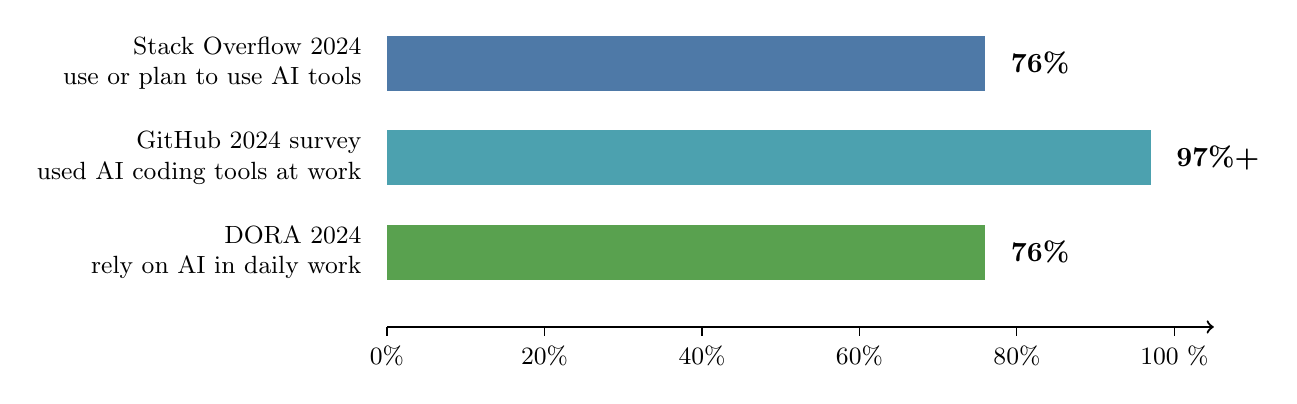
\begin{tikzpicture}[font=\small]
    \definecolor{adoptblue}{RGB}{78,121,167}
    \definecolor{adoptteal}{RGB}{76,161,175}
    \definecolor{adoptgreen}{RGB}{89,161,79}

    \draw[->, thick] (0,0) -- (10.5,0);

    \foreach \x/\label in {
      0/0,
      2/20,
      4/40,
      6/60,
      8/80,
      10/100
    }{
      \draw (\x,0) -- (\x,-0.12);
      \node[below] at (\x,-0.12) {\label\%};
    }

    \fill[adoptblue] (0,3.0) rectangle (7.6,3.7);
    \fill[adoptteal] (0,1.8) rectangle (9.7,2.5);
    \fill[adoptgreen] (0,0.6) rectangle (7.6,1.3);

    \node[anchor=east, align=right] at (-0.2,3.35) {Stack Overflow 2024\\use or plan to use AI tools};
    \node[anchor=east, align=right] at (-0.2,2.15) {GitHub 2024 survey\\used AI coding tools at work};
    \node[anchor=east, align=right] at (-0.2,0.95) {DORA 2024\\rely on AI in daily work};

    \node[anchor=west, font=\bfseries] at (7.8,3.35) {76\%};
    \node[anchor=west, font=\bfseries] at (9.9,2.15) {97\%+};
    \node[anchor=west, font=\bfseries] at (7.8,0.95) {76\%};
  \end{tikzpicture}%
  }
  \caption{Selected survey results illustrating the prevalence of \ac{AI}-assisted software development. The figures are based on different populations and question formulations, so they should be read as trend indicators rather than directly comparable measurements.}
  \label{fig:ai_dev_adoption}
\end{figure}


  \subsection{Potential benefits}
  One important reason for the rapid adoption of \ac{AI} tools is that they appear to offer real gains in productivity and workflow support. These gains do not necessarily mean that the model replaces the developer. Rather, the benefit often lies in assisting with time-consuming or repetitive tasks such as code completion, boilerplate generation, refactoring suggestions, test drafting, documentation support, and codebase exploration. This can allow the developer to spend a greater proportion of time on design decisions, debugging strategy, and evaluation of alternative solutions.

  Recent empirical work also suggests that these benefits are not only anecdotal. Controlled and field-based studies indicate that access to coding assistants can increase the rate at which software tasks are completed, although the size of the effect depends on context, task type, and developer experience \cite{cuiEffectsGenerativeAI2025}. At the same time, many studies and reports frame the benefit less as fully autonomous programming and more as augmented development, where the developer remains responsible for understanding and validating the result \cite{staffSurveyRevealsAIs2023,CodexAICoding,CodexNowGenerally2026}.

  \subsection{Limitations}
  At the same time, increased adoption does not imply unconditional trust. One of the clearest themes in recent literature and survey material is that developers often find \ac{AI} useful while still being skeptical of its output \cite{AI2024Stack,wangInvestigatingDesigningTrust2023}. This skepticism is well justified. \ac{AI}-generated code may be syntactically correct while still misunderstanding requirements, introducing subtle bugs, using poor abstractions, or suggesting insecure solutions. It can also create the false impression that a difficult problem has been solved simply because a fluent-looking answer has been produced.

  For this reason, the value of \ac{AI} in software development depends heavily on verification, domain understanding, and responsible use. A developer who relies on \ac{AI} without understanding the surrounding system risks turning the tool into a crutch. By contrast, a developer who already understands the problem domain can use \ac{AI} more effectively as an assistant: to accelerate drafting, explore alternatives, and reduce routine effort while still retaining control of the technical decisions \cite{wangInvestigatingDesigningTrust2023}.

  This perspective aligns well with the idea of appropriate trust. The goal is not to reject \ac{AI}, but to use it with enough understanding that its contributions can be evaluated critically. In other words, \ac{AI} can improve development speed and convenience, but only if the human developer remains responsible for interpretation, validation, and final judgment \cite{AI2024Stack,wangInvestigatingDesigningTrust2023,DORAAccelerateState}.

  \subsection{Relevance to this thesis}
  In this thesis, \ac{AI} is not treated as a replacement for software engineering work, but as a tool that may support the development process. This is the reason the first two iterations were developed without \ac{AI} assistance. Doing the early work manually helped establish a basic understanding of the musical domain, the program structure, and the design trade-offs involved in the project. Without that foundation, it would be much harder to judge whether \ac{AI}-generated suggestions were correct, useful, or aligned with the goals of the system.

  The third iteration therefore uses \ac{AI} in a more deliberate way. By that stage, the project has already accumulated enough structure and domain knowledge that \ac{AI} can be used more productively as a development aid. This makes it possible to evaluate not only whether the final system improves, but also whether \ac{AI} is practically useful in a constrained, iterative, technically demanding development process. The aim is thus not to let \ac{AI} carry the work, but to investigate whether it can function as a tool for assisting and streamlining the work.

